The Blelloch scan \cite{BlellochTR90} is based on a balanced tree, consisting of two phases, the up-sweep phase and the down-sweep phase. A visual representation of the Blelloch scan is seen in \cref{fig:scan_blelloch}. 

\begin{figure}[ht]
	\centering
	\fbox{
		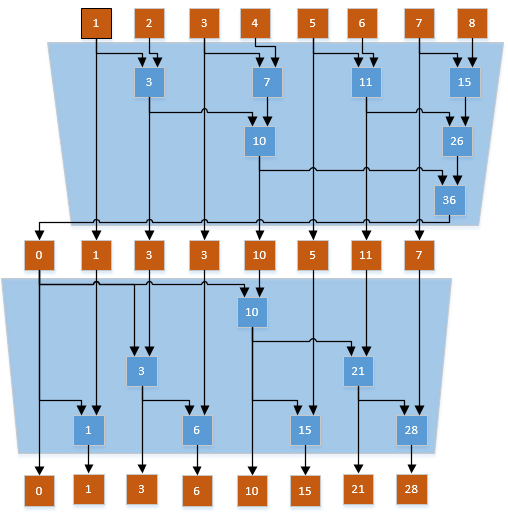
\includegraphics[width=0.5\textwidth]{figs/algorithm/scan_blelloch.png}}
	\caption{Blelloch exclusive scan, first part is the up-sweep , second is the down-sweep}
	\label{fig:scan_blelloch}
\end{figure}

The first phase, the up-sweep, is a reduction as described in \cref{sec:al_reduction}. The reduction will only produce the partial tree summations, resulting in the need for the down-sweep. The down-sweep starts with the identity element and goes from the root to the leaves, opposed to the up-sweep. The Blelloch scan in its representation is an exclusive scan, but can be made inclusive through shifting, or by implementation as seen in \cref{fig:scan_inclusive}.

\begin{figure}[ht]
	\centering
	\fbox{
		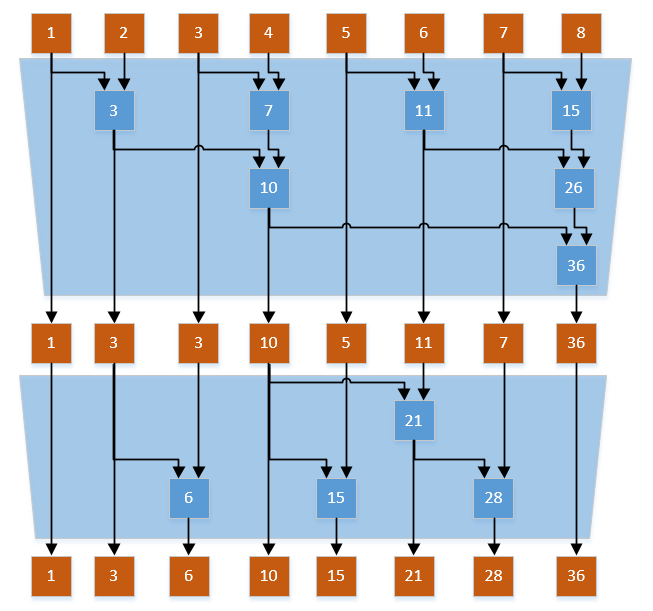
\includegraphics[width=0.5\textwidth]{figs/algorithm/scan_blelloch_inclusive.png}}
	\caption{Inclusive representation of the Blelloch scan}
	\label{fig:scan_inclusive}
\end{figure}

The up-sweep and down-sweep in their inclusive form is equal in terms of step and work complexity. The up-sweep is a reduction, with $\mathcal{O}(n)$ work and $\mathcal{O}(log~n)$ steps, meaning the Blelloch scan has $\mathcal{O}(2n)$ work and $\mathcal{O}(2~log~2)$ step complexity. The Blelloch scan is step efficient compared with the serial implementation, but not as step efficient as the Hillis/Steele scan. On the other hand it is more work efficient than the Hillis/Steele. In a case where there are more array elements than processors the Blelloch scan would prove faster than the Hillis/Steele. It is therefore application specific which scan should be used.